
\item A point moves rectilinearly in one direction. Fig. 1.1 shows the distance \( s \) traversed by the point as a function of the time \( t \).
    \begin{center}
        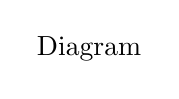
\begin{tikzpicture}
            \node at (0, 0) {Diagram}; % Replace this with the actual TikZ code for the diagram.
        \end{tikzpicture}
    \end{center}
Using the plot find:
\begin{itemize}
    \item the average velocity of the point during the time of motion;
    \item the maximum velocity;
    \item the time moment \( t_0 \) at which the instantaneous velocity is equal to the mean velocity averaged over the first \( t_0 \) seconds.
\end{itemize}
